
\begin{figure}
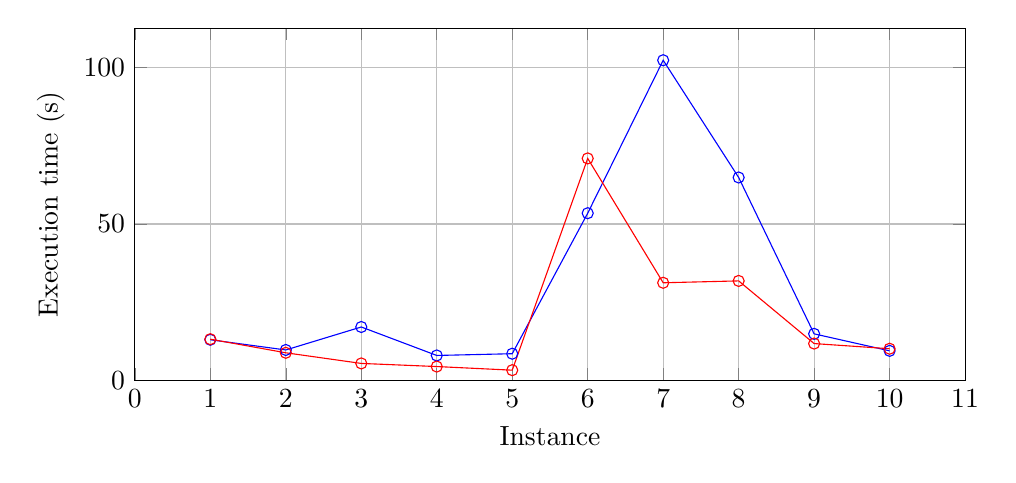
\begin{tikzpicture}
	\begin{axis}[width=\textwidth,height=40ex,
		xlabel=Instance,
		ylabel=Execution time (s), xmin=0, ymin=0, grid=both]
	
	
\addplot[mark=o,color=blue] coordinates {
(1, 12.96708331)
(2, 9.704563172)
(3, 17.056811547)
(4, 7.944795782)
(5, 8.505190252)
(6, 53.456992427)
(7, 102.392618933)
(8, 64.881486922)
(9, 14.86064378)
(10, 9.421963416)
};

\addplot[mark=o,color=red] coordinates {
(1, 13.152454848)
(2, 8.8)
(3, 5.4)
(4, 4.4)
(5, 3.24)
(6, 70.99)
(7, 31.2)
(8, 31.8)
(9, 11.75)
(10, 10.1)
};
\end{axis}

\end{tikzpicture}%
\caption{Execution time for Gurobi on all instances with P1 (in red) and P3 (in blue)}
\end{figure}
